\documentclass[titlepage,a4paper]{article}

\usepackage{a4wide}
\usepackage[colorlinks=true,linkcolor=black,urlcolor=blue,bookmarksopen=true]{hyperref}
\usepackage{bookmark}
\usepackage{fancyhdr}
\usepackage[spanish]{babel}
\usepackage[utf8]{inputenc}
\usepackage[T1]{fontenc}
\usepackage{graphicx}
\usepackage{float}

\pagestyle{fancy} % Encabezado y pie de página
\fancyhf{}
\fancyhead[L]{Apuntes Análisis de la información}
\fancyhead[R]{1C2021}
\renewcommand{\headrulewidth}{0.4pt}
\fancyfoot[C]{\thepage}
\renewcommand{\footrulewidth}{0.4pt}

\begin{document}
\begin{titlepage} % Carátula
	\hfill
\includegraphics[width=6cm]{logofiuba.jpg}
    \centering
    \vfill
    \Huge \textbf{Apuntes de análisis de la información}
    \vskip2cm
    \Large [7509] Análisis de la información\\
    Curso González \\
    1C 2021 
    \vfill
    \begin{tabular}{ | l | l | } % Datos del alumno
      \hline
      Alumno: & Grassano, Bruno \\ \hline
      Número de padrón: & 103855 \\ \hline
      Email: & bgrassano@fi.uba.ar \\ \hline
  	\end{tabular}
    \vfill
    \vfill
\end{titlepage}

\tableofcontents % Índice general

\newpage

\section{Introducción}\label{sec:intro}
El presente archivo contiene los apuntes que fueron tomados a lo largo de la cursada de la materia análisis de la información (7509) en el curso del profesor González.

% Grupos 5/6
% Final exposición de TP para coloquio. Evaluación de la exposición, calidad del trabajo, presentación, algunas preguntas teóricas individuales (solo sobre lo de los lunes)
% Nota final: Conceptual (Alejandro sobre el trabajo) + Exposición + Respuestas a preguntas teóricas


\section*{Primera clase}

    \begin{itemize}
        \item Introducción a la Ing. Software: Definiciones y metodología
        \item Modelos bajo el paradigma de OO
        \item Modelos de objetivos: Objetivo, alcance y hipótesis de un sistema
    \end{itemize}

\section{Introducción a la Ing. Software}
Definición: \textit{'Es la aplicación de un enfoque sistemático disciplinado y cuantificable al desarrollo, operación y mantenimiento de productos de software.'} (IEEE 1993) (Enfoque ingenieril)

\medskip

Otra definición: \textit{'Comprende principios y \textbf{metodologías} para desarrollar, operar y mantener software de calidad.'}


\subsection{Metodologías}
Contiene 3 partes. Los modelos, procesos, y las herramientas de un desarrollo de software. Estos son específicos a una metodología.

    \begin{itemize}
        \item Los modelos necesitan de un lenguaje de modelado $\rightarrow$ UML.
        \item Los procesos son \textit{XP, SCRUM, RUP, etc}
        \item Herramientas \textit{Suite Rational}
    \end{itemize}
    
    \begin{figure}[!htb]
        \centering
        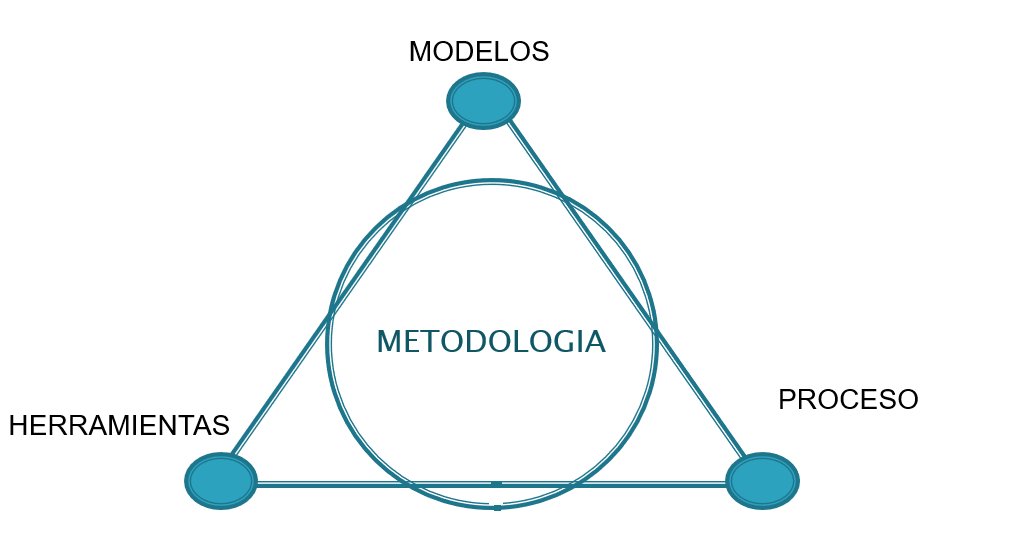
\includegraphics[width=0.8\textwidth]{Imagenes/Metodologias.png}
        \caption{Composición de una metodología}
    \end{figure}

\subsection{Modelos}
\subsubsection*{¿Que es un modelo?}
Es una simplificación de la realidad. Como la realidad es compleja le aplicamos abstracción, para incluir elementos que tienen mucha influencia y omitir los relevantes.

\subsubsection*{¿Para que sirve un modelo?}
    \begin{itemize}
        \item Para comprender mejor el sistema que estamos desarrollando.
        \item Para poder comunicarnos, con el cliente y el equipo de diseño.
        \item Visualizar y controlar rápidamente la arquitectura del sistema.
        \item Gestionar el riesgo de un proyecto. \textit{Calidad, plazos, y presupuesto}
    \end{itemize}

\subsubsection*{Etapas}
    \begin{itemize}
        \item Captura de requerimientos. \textit{Reuniones con cliente, cuestionarios, focus groups,...}
        \item Análisis de requerimientos: Es el ¿Que se necesita? \textit{Modelos de casos de uso, historias de usuario,...}
        \item Diseño: Es el ¿Como voy a hacer? \textit{Modelos de clases, de objetos, de despliegue,...}
        \item Construcción. \textit{Programación, integración de componentes...}
        \item Pruebas. \textit{Pruebas de sistema, unitarias, de usuario, de integración}
        \item Entrega. \textit{Despliegue del producto a los usuarios}
        \item Mantenimiento. \textit{Correctivo (Corregir defectos de diseño) y evolutivo (Adaptar a los nuevos procesos)}
    \end{itemize}

\subsubsection{Principios de la modelización}
    \begin{itemize}
        \item La elección de que modelos crear tiene una gran influencia sobre como se aborda un problema y como se da la solución.
        \item Tienen distintos niveles de precisión.
        \item Los mejores modelos tienen que estar ligados a la realidad.
        \item Un único modelo no es suficiente.
        \item Tener un Objetivo y alcance claro.
    \end{itemize}

\subsubsection{Beneficios de la modelización}
    \begin{itemize}
        \item Forma de visualizar necesidades y requerimientos contra costos reales antes de comenzar el desarrollo.
        \item Se trabaja en un alto nivel de abstracción
    \end{itemize}


\subsubsection*{Enfoques}
    \begin{itemize}
        \item Algorítmico
        \item Orientado a objetos
    \end{itemize}

\subsection{Paradigma orientado a objetos}
    \begin{itemize}
        \item Esta basado en la creación de componentes reutilizables.
        \item Construcción de software mas rápida y dinámica.
        \item Facilita la creación de prototipos.
    \end{itemize}

\subsection{UML}
Es un \textbf{lenguaje} estándar para escribir 'planos' de software. Lenguaje para visualizar, especificar, construir y documentar sistemas bajo el paradigma de orientación a objetos. Se utiliza desde el inicio hasta el fin del proyecto.
\textbf{No} es una \textbf{metodología}.

    \begin{figure}[!htb]
        \centering
        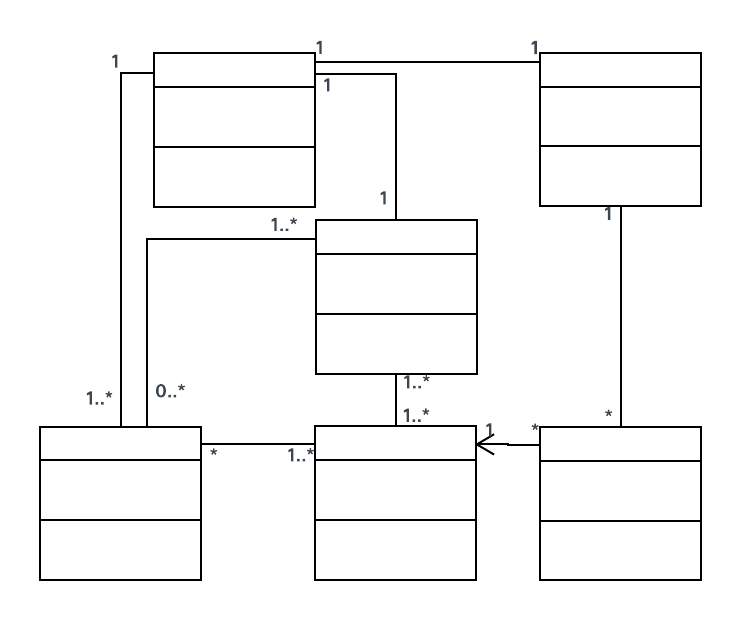
\includegraphics[width=0.5\textwidth]{Imagenes/UML.png}
    \end{figure}

\subsection*{Aspectos del modelado}
    \begin{itemize}
        \item Modelado funcional o de comportamiento. \textit{Historias de usuario}
        \item Modelado estático o estructural. \textit{Diagrama de clases}
        \item Modelado dinámico. \textit{Diagramas de interacción, secuencia}
    \end{itemize}

\subsection{Procesos de desarrollo de software}

Tiene que responder a 4 preguntas: ¿Quien lo hace?, ¿Que lo hace?, ¿Como lo hace?, ¿Cuando lo hace?
De forma tal de obtener un producto de calidad, dentro de plazos y presupuestos predecibles.

\section{Modelo de Objetivos}
\subsection{Objetivo del sistema}
Define lo que el sistema va a hacer (objetivo).
Es una descripción breve con alto nivel de abstracción, sobre \textbf{que} se requiere automatizar con el sistema, declarando los 'macroprocesos'.

\textit{Ej.
El sistema esta dirigido a administrar las ventas de la empresa, incluyendo la gestión de los pedidos del stock y la facturación de las mismas'.}

Macroprocesos involucrados: Gestión de pedidos, gestión de stock, gestión de facturación.

\subsection{Alcance del sistema}
Muestra los limites del objetivo(alcance). Para cada 'macroprocesos' hay que indicar las funcionalidades que el sistema va a contemplar,
dejando bien en claro que funcionalidades están \underline{dentro}/\underline{fuera} del alcance

Formato típico de un análisis del alcance.



\begin{table}[]
\begin{center}
\begin{tabular}{|l|l|c|}
\hline
\multicolumn{1}{|c|}{Macroproceso} & \multicolumn{1}{c|}{Funcionalidades} & Alcance \\ \hline
\textit{Nombre macroproceso}      & \textit{Nombre funcionalidad}       & \textit{Si/No} \\ \hline
 \multicolumn{1}{|c|}{...}          & \multicolumn{1}{c|}{...}            & ...            \\ \hline
\end{tabular}
\end{center}
\end{table}


\subsection{Hipótesis o supuestos funcionales}
Establece premisas o restricciones a tener en cuenta. (hipótesis)
Pueden ser establecidas por políticas de la empresa, normativas legales. Supuestos iniciales establecidos por el analista (deben ser verificados después por el cliente). No son requerimientos relevados, sino que complementan a los mismos.

Estos pueden darse por falta de relevamiento por determinadas circunstancias. \textit{Ej. El cliente se lo olvido, es trivial, no lo sabe, lo oculta}

\section{Caso de estudio: Airbus A320}

Habilitar la aceleración en reversa. El avión al momento de frenar activa este mecanismo, abriendo unos alerones en las turbinas.

El software: el piloto acciona el comando, ocurre un servo-mecanismo que abre los alerones. Caso de error a evitar, si el piloto lo acciona volando, tiene que haber algún mecanismo que detecte que el avión este en el piso. Se agrego un sensor de giro de ruedas, que detecta cuando giran en el piso y habilita la reversa del sistema que acciono el piloto.

El software salio de esta forma, pero tenia un problema, el avión estaba aterrizando, pero en caso de que la pista tenga hielo se producía un bloqueo y la rueda patinaba en vez de girar. Esto pasó debido a que no se contemplo en el universo en estudio.

Se debería de haber tenido en cuenta el sensor de giro, de peso, y de altura.

Sistema de estudio: software, los 3 sensores, el servo-mecanismo reversa.


\section*{Segunda clase}

    \begin{itemize}
        \item Modelo de negocio.
        \item Mapa de procesos.
        \item Mapa de sistemas.
        \item Diagrama de actividad.
    \end{itemize}

\section{Modelo de negocio}

\subsection{Mapa de procesos}
    \begin{itemize}
        \item Modeliza los procesos que una organización tiene para llevar adelante sus funciones.
        \item Permite entender la organización/negocio.
        \item Es un modelo matricial, modela los principales macroprocesos necesarios para el funcionamiento del negocio/empresa.
        \item Columnas: áreas del negocio. \textit{Ej. Estrategia y planificación, operación, previsión, assurance, billing}
        \item Filas: visión por capas. \textit{Ej. cliente, servicio, recurso, enterprise}
    \end{itemize}
    
    
    Conocer aquellos que vamos a automatizar, mas aquellos que interaccionan con el mismo.
    
\subsection{Mapa de sistemas}
    \begin{itemize}
        \item Modelo matricial: incluye los sistemas que dan soporte a los procesos de negocio.
        \item Columnas: áreas del negocio
        \item Filas: visión por capas
    \end{itemize}

Mapea determinados macroprocesos, y va diciendo cuales son los sistemas que van a automatizar los macroprocesos (mapa de sistemas) Puede ser mapeo 1 a 1, 1 a N, N a 1.

\subsection{Diagrama de actividad}
    \begin{itemize}
        \item Modeliza una secuencia de actividades en un escenario determinado. Modelo gráfico.
        \item Esta compuesto por un grafo dirigido. Los nodos son actividades, y los arcos (dirigidos) representan la transición entre actividades.
        \item Actividad de inicio, es única (circulo relleno) 
        \item Actividades de fin, puede haber varias (circulo con borde)
        \item El rombo (bifurcación) es de decisión. Indica caminos alternativos, elegidos según el valor de alguna expresión, surgida de un análisis que se lleva a cabo en una actividad.
        \item Barra de sincronización, agregar la barra indica que para que inicie otra actividad, tienen que haber finalizado todas las actividades que vayan a la barra.
        \item Dividiendo como columnas, agregar los responsables de cada actividad, quien las ejecuta. (Las 'Swimming lines', carriles, dividen las actividades')
        \item Estos diagramas no muestran temporalidad, esto esta en diagramas de secuencia.
        \item No muestran requisitos NO funcionales.
        \item Muy claro para comunicarse con el cliente y asegurarse de que se entendieron los requerimientos.
        \item Buen punto de partida para generar el modelo de comportamiento.
        \item Tipos de escenarios
        \begin{itemize}
            \item Global, contiene todos los procesos de negocio del universo en estudio.
            \item Parte del negocio, contiene algunos procesos de negocio del universo en estudio
            \item Un solo proceso de negocio, tiene todas las actividades de ese proceso.
            \item Regla de negocio, son las actividades de una regla de negocio.
        \end{itemize}
    \end{itemize}

    \begin{figure}[!htb]
        \centering
        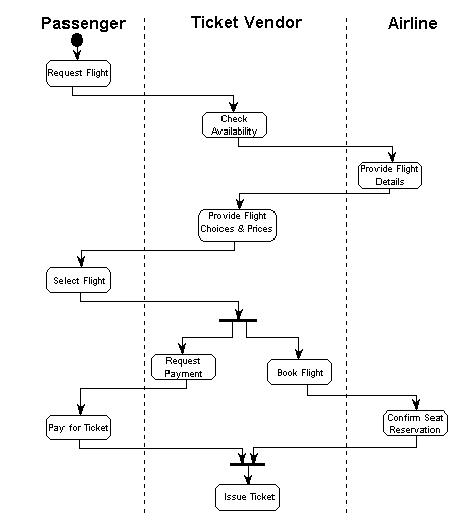
\includegraphics[width=0.7\textwidth]{Imagenes/DiagramaActividad.png}
        \caption{Diagrama de actividad. Notar las diferentes entidades: Actores, actividad de inicio (de fin falta), las secuencias, barras de sincronización.}
    \end{figure}

Una actividad esta compuesta por un conjunto de tareas a ser realizadas. Verbo $+$ objeto, \textit{ej. verificar pedido}. No hay que asociarlas con actividades físicas, si con procesos y/o reglas de negocio que luego podrán ser (o no) automatizadas.










\newpage





\section{Bibliografía de la materia}

\begin{itemize}
    \item The Unified Modeling Language Reference Manual, Rumbauch, Jacobson, Booch
    \item The Unified Software Development Process, Rumbauch, Jacobson, Booch
    \item UML distilled, Third Edition, Fowler
\end{itemize}

\end{document}
